\documentclass[]{article}
\usepackage{graphicx}
\usepackage{subfig}

%opening
\title{
	Artificial Composer\\
	\texttt{}\\
	\large Intelligent Information Systems}

\author{Paulina Szwed}

\begin{document}

\maketitle

\section{Introduction}

The objective of the project was to create an intelligent information system
that is able to generate music on its own. Although content generation is not one
of the main usecases for the information systems, this subject is progressing
very quickly, mainly because of the possibilities created by deep neural networks.

One of the techniques to build such systems that often gives very promising 
results is the use of generative adversarial networks (GAN). GAN is a compound system made of two neural networks - the generator and the discriminator. The discriminator is the component that determines whether the content shown to it is real or generated artificially (fake). The generator tries to deceive the discriminator by creating more and more realistic content. During my experiments I used three variants of GAN architecture in order to create a system generating the most realistic music.

\section{Experiments}

Experiments were conducted on different types of GAN but every one of them used the same training loop. Two of them were trained on songs from Maestro dataset \cite{hawthorne2018enabling} from 2018, the last experiments used songs by Queen from \cite{queenmidisongs}. All experiments used files in MIDI format, but converted into different representations. 

\subsection{Training loop}

The training loop was divided into two stages. First, the discriminator was trained on a whole epoch of real samples (with expected output of ones) and a whole epoch of fake samples (with expected output of zeros). Then, the generator was trained by exposing the combined system with frozen discriminator weights to an epoch of fake samples, but with expected output of ones. 

Before the actual training loop I introduced a pretraing stage, to initially enhance the performance of the generator - the pretraining stage was only training the combined system like in the second stage of the main training loop.

In every case I trained the models on batches of 8 samples each and I performed 5 epochs of pretraining.

\subsection{Models}

During my reserach I tried out different models for generators and discriminators. I also used different methods for representing information from the training set. 

\subsubsection{One Hot Encoding DCGAN}

At first I used a DCGAN (deep convolutional generative adversarial networks \cite{dcgan}). In this model the discriminator processed genetrated content as images, using convolutional layers and the generator uses deconvolution to create an image from vector of random numbers. Table \ref{ohe-dcgan} shows detailed description of the model that I trained.

\begin{table}[h!]
	\centering
	\begin{tabular}{|r|c|c|}
		\hline
		\multicolumn{1}{|c|}{\textbf{Index}} & \textbf{Layer type} & \textbf{Description}                      \\ \hline
		\multicolumn{3}{|c|}{\textbf{Generator}}                                                               \\ \hline
		1                                    & Dense               & 8192 neurons                              \\ \hline
		2                                    & Leaky ReLU          & alpha 0.2                                 \\ \hline
		3                                    & Reshape             & Reshaping into vector 8 x 8 x 128         \\ \hline
		4                                    & Deconvolution       & 64 filters 4x4                            \\ \hline
		5                                    & Leaky ReLU          & alpha 0.2                                 \\ \hline
		6                                    & Deconvolution       & 64 filters 4x4                            \\ \hline
		7                                    & Leaky ReLU          & alpha 0.2                                 \\ \hline
		8                                    & Deconvolution       & 64 filters 4x4                            \\ \hline
		9                                    & Leaky ReLU          & alpha 0.2                                 \\ \hline
		10                                   & Convolution         & 1 filter 7x7, sigmoid activation function \\ \hline
		\multicolumn{3}{|c|}{\textbf{Discriminator}}                                                                    \\ \hline
		1                                    & Convolution         & 128 filters 5x5                           \\ \hline
		2                                    & Leaky ReLU          & alpha 0.2                                 \\ \hline
		3                                    & Dropout             & dropout factor 0.2                        \\ \hline
		4                                    & Convolution         & 64 filters 3x3                            \\ \hline
		5                                    & Leaky ReLU          & alpha 0.2                                 \\ \hline
		6                                    & Dropout             & dropout factor 0.2                        \\ \hline
		7                                    & Convolution         & 32 filters 3x3                            \\ \hline
		8                                    & Leaky ReLU          & alpha 0.2                                 \\ \hline
		9                                    & Dropout             & dropout factor 0.2                        \\ \hline
		10                                   & Flatten             &                                           \\ \hline
		11                                   & Dense               & 1 neuron, sigmoid activation function     \\ \hline
	\end{tabular}
	\caption{Simple one-hot encoding DC GAN structure}
	\label{ohe-dcgan}
\end{table}

The representation for the music I used in the first experiment was a matrix created from notes in MIDI file. Each note was a integer value between 0 and 127, so I decided to build an matrix of size 127 on 127 pixels in which every row represented one note and it contained 127 notes long fragment of a song. For representing notes I used one-hot encoding, which means that I converted the value to an index of a element in the matrix row, filled it with value 1.0 and the rest of them with zeros.

The training process is shown in figures \ref{fig:simplecnn-loss} and \ref{fig:simplecnn-acc}. 

\begin{figure}[!h]
	\centering
	\subfloat[Loss during training]{
		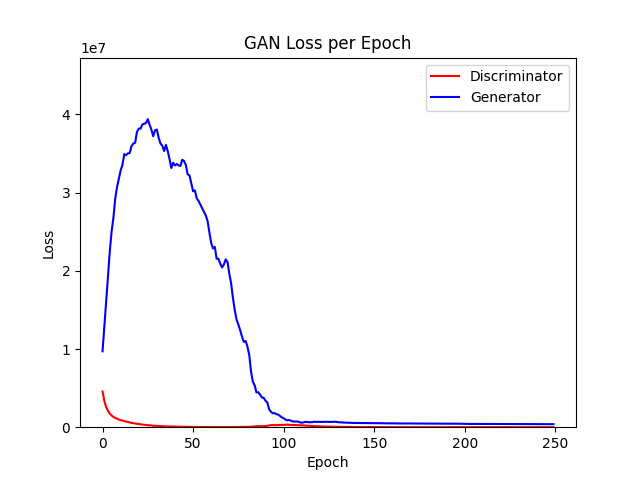
\includegraphics[width=0.49\textwidth]{img/simple-cnn-dcnn-GAN_GAN_Loss_per_Epoch_final.png}
		\label{fig:simplecnn-loss}
	}    
	\subfloat[Discriminator accuracy during training]{
		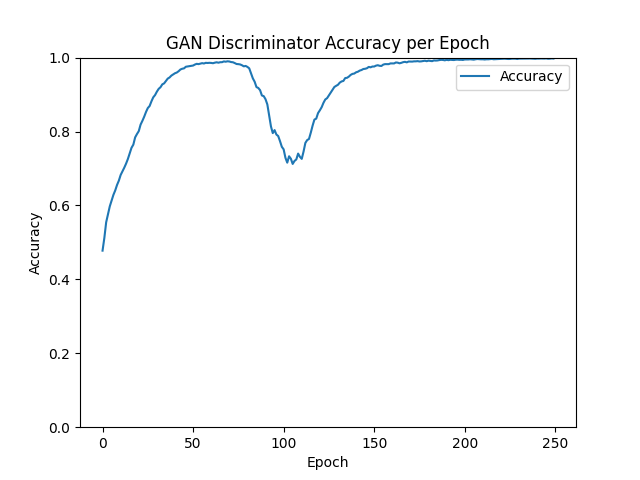
\includegraphics[width=0.49\textwidth]{img/simple-cnn-dcnn-GAN_GAN_Accuracy_per_Epoch_final.png}
		\label{fig:simplecnn-acc}
	}
	\caption{Loss and accuracy during training of simple one-hot encoding DCGAN}
\end{figure}

The results shown that such architecture can be a mechanism to create some kind of music, but it's possibilities were limited to simple sounds - one-hot encoding does not allow to use chords. There is also only one instrument in those generated songs.

\subsubsection{LSTM-based GAN}

Next I used a generator made of densily connected layers and a discriminator that contained 2 layers of LSTM cells. I was hoping that LSTM's "memory" will improve performance by better perception of sequential patterns in songs. Music was represented as a sequence of numerical values indicating notes of the song. The detailed description of the layers is provided in table \ref{lstm-gan}. 

\begin{table}[]
	\centering
	\begin{tabular}{|r|c|c|}
		\hline
		\multicolumn{1}{|c|}{\textbf{Index}} & \textbf{Layer type} & \textbf{Description}                  \\ \hline
		\multicolumn{3}{|c|}{\textbf{Generator}}                                                           \\ \hline
		1                                    & Dense               & 256 neurons                           \\ \hline
		2                                    & Leaky ReLU          & alpha 0.2                             \\ \hline
		3                                    & Batch Normalization & momentum 0.8                          \\ \hline
		4                                    & Dense               & 256 neurons                           \\ \hline
		5                                    & Leaky ReLU          & alpha 0.2                             \\ \hline
		6                                    & Batch Normalization & momentum 0.8                          \\ \hline
		7                                    & Dense               & 512 neurons                           \\ \hline
		8                                    & Leaky ReLU          & alpha 0.2                             \\ \hline
		9                                    & Batch Normalization & momentum 0.8                          \\ \hline
		10                                   & Dense               & 16384 neurons                         \\ \hline
		11                                   & Reshape             & reshaping into matrix 128 x 128       \\ \hline
		\multicolumn{3}{|c|}{\textbf{Discriminator}}                                                       \\ \hline
		1                                    & LSTM                & 128 cells                             \\ \hline
		2                                    & Bidirectional LSTM  & 512 cells                             \\ \hline
		3                                    & Dense               & 256 neurons                           \\ \hline
		4                                    & Leaky ReLU          & alpha 0.2                             \\ \hline
		5                                    & Batch Normalization & momentum 0.8                          \\ \hline
		6                                    & Dense               & 128 neurons                           \\ \hline
		7                                    & Leaky ReLU          & alpha 0.2                             \\ \hline
		8                                    & Batch Normalization & momentum 0.8                          \\ \hline
		9                                    & Dense               & 64 neurons                            \\ \hline
		10                                   & Leaky ReLU          & alpha 0.2                             \\ \hline
		11                                   & Batch Normalization & momentum 0.8                          \\ \hline
		12                                   & Dense               & 1 neuron, sigmoid activation function \\ \hline
	\end{tabular}
	\caption{LSTM-based GAN structure}
	\label{lstm-gan}
\end{table}

Figures \ref{fig:lstmgan-loss} and \ref{fig:lstmgan-acc} shows the training process. As we can see, the LSTM-based architecture had troubles with short learning span. It's noticeable that this system quickly degraded and music generated by it becomes a sequence of minimum and maximum values. Those troubles were probably caused by exploding gradients problem. 

\begin{figure}[!h]
	\centering
	\subfloat[Loss during training]{
		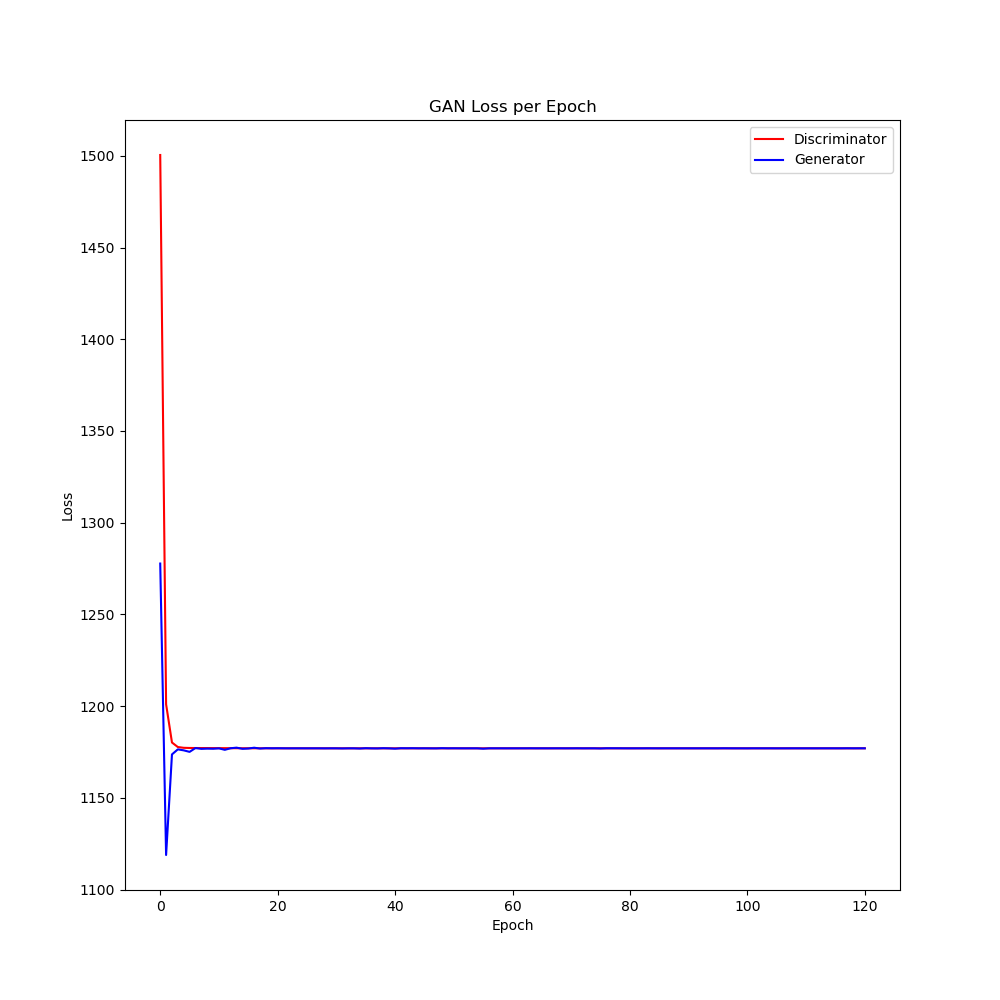
\includegraphics[width=0.49\textwidth]{img/2021_02_08_21_47_26_midi-notes-lstm-gan-scalec_GAN_Loss_per_Epoch_epoch_120.png}
		\label{fig:lstmgan-loss}
	}    
	\subfloat[Discriminator accuracy during training]{
		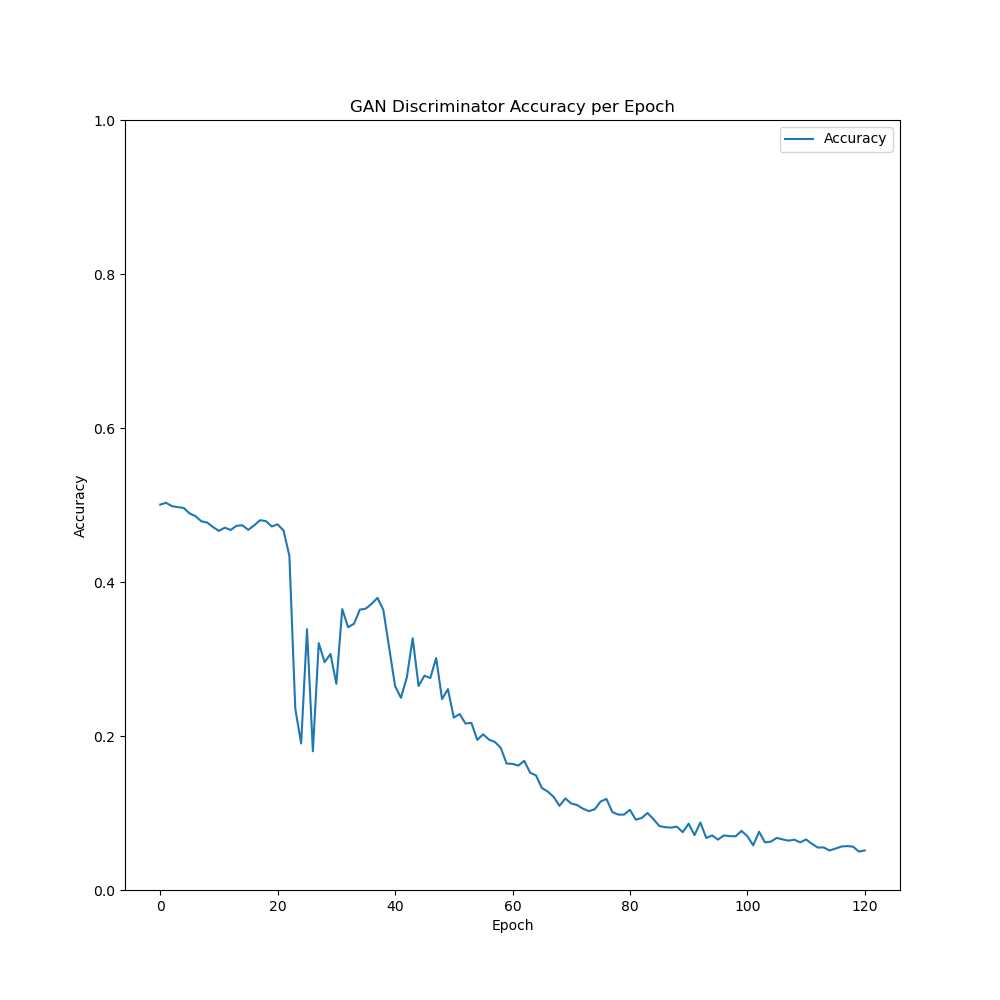
\includegraphics[width=0.49\textwidth]{img/2021_02_08_21_47_26_midi-notes-lstm-gan-scalec_GAN_Accuracy_per_Epoch_epoch_120.png}
		\label{fig:lstmgan-acc}
	}
	\caption{Loss and accuracy during training of LSTM-based GAN}
\end{figure}

LSTM-based GAN can be a system for music generation, but it has the same limitations as DCGAN with one-hot encoding. The exploading gradients problem made it impossible to aquire more realistic results, but it still did generate some interesting samples in which we can hear some repeating patterns. 

\subsubsection{Pianoroll-based DCGAN}

At the next stage of the experiments I went back to the DCGAN architecture but with different approach to representation of music. I used a pianoroll format and converted it into a matrix that had 3 channels (depth equal to 3) so that I could place there an information on chords played by different instruments and even drums. Table \ref{pianoroll-dc-gan} shows detailed description of layers in the system.

\begin{table}[h!]
	\centering
	\begin{tabular}{|r|c|c|}
		\hline
		\multicolumn{1}{|c|}{\textbf{Index}} & \textbf{Layer type} & \textbf{Description}                  \\ \hline
		\multicolumn{3}{|c|}{\textbf{Generator}}                                                           \\ \hline
		1                                    & Dense               & 8912 neurons                          \\ \hline
		2                                    & Leaky ReLU          & alpha 0.2                             \\ \hline
		3                                    & Reshape             & reshaping to matrix 8 x 8 x 128       \\ \hline
		4                                    & Deconvolution       & 64 filters 4x4                        \\ \hline
		5                                    & Batch Normalization & momentum 0.8                          \\ \hline
		6                                    & Leaky ReLU          & alpha 0.2                             \\ \hline
		7                                    & Deconvolution       & 64 filters 4x4                        \\ \hline
		8                                    & Batch Normalization & momentum 0.8                          \\ \hline
		9                                    & Leaky ReLU          & alpha 0.2                             \\ \hline
		10                                   & Deconvolution       & 64 filters 4x4                        \\ \hline
		11                                   & Batch Normalization & momentum 0.8                          \\ \hline
		12                                   & Leaky ReLU          & alpha 0.2                             \\ \hline
		13                                   & Convolution         & 3 filters 7x7                         \\ \hline
		\multicolumn{3}{|c|}{\textbf{Discriminator}}                                                       \\ \hline
		1                                    & Convolution         & 128 filters 5x5                       \\ \hline
		2                                    & Leaky ReLU          & alpha 0.2                             \\ \hline
		3                                    & Convolution         & 128 filters 5x5                       \\ \hline
		4                                    & Leaky ReLU          & alpha 0.2                             \\ \hline
		5                                    & Convolution         & 64 filters 3x3                        \\ \hline
		6                                    & Leaky ReLU          & alpha 0.2                             \\ \hline
		7                                    & Convolution         & 32 filters 3x3                        \\ \hline
		8                                    & Leaky ReLU          & alpha 0.2                             \\ \hline
		9                                    & Flatten             &                                       \\ \hline
		10                                   & Dense               & 1 neuron, sigmoid activation function \\ \hline
	\end{tabular}
	\caption{Pianoroll DCGAN structure}
	\label{pianoroll-dc-gan}
\end{table}

Training process is shown in figures \ref{fig:pianoroll-loss} and \ref{fig:pianoroll-acc}. As we can see it was longest training process and it did not lead to exploading or vanishing gradients. 

\begin{figure}[!h]
	\centering
	\subfloat[Loss during training]{
		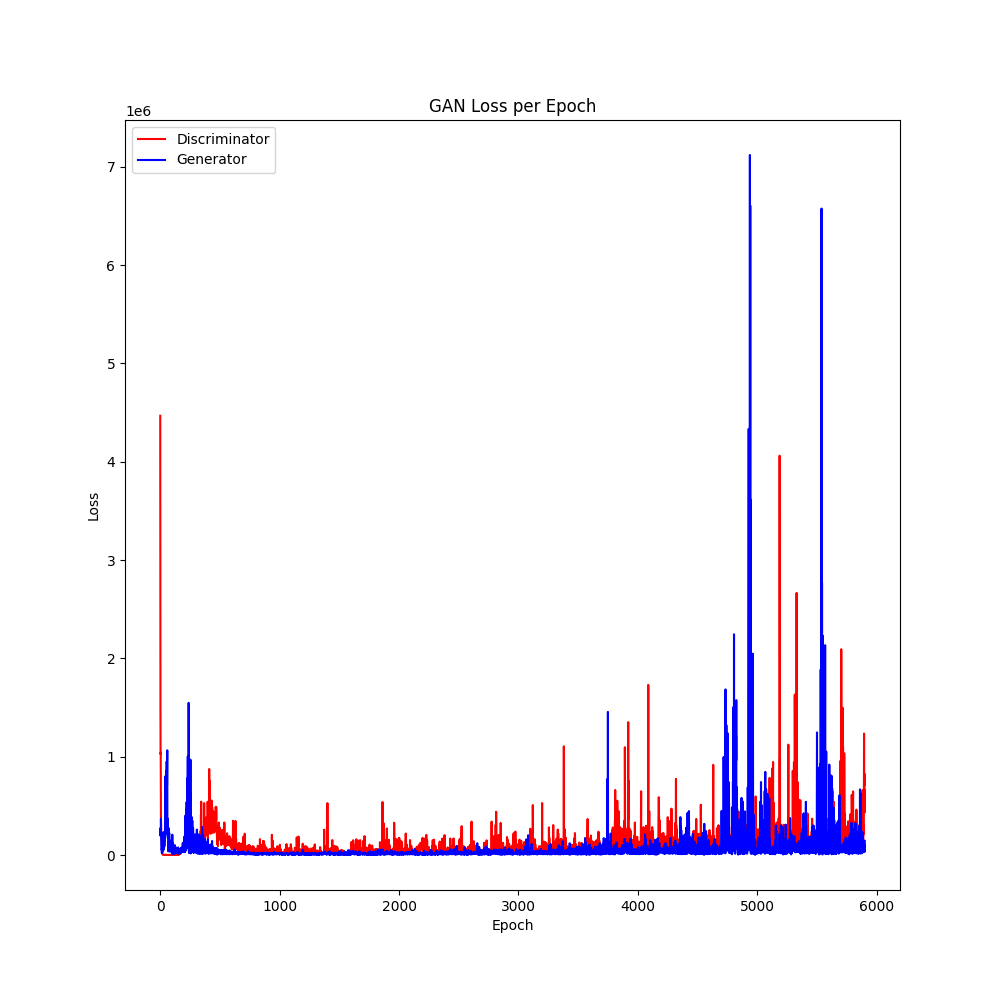
\includegraphics[width=0.49\textwidth]{img/2021_01_31_22_56_40_pianoroll-DC-GAN_GAN_Loss_per_Epoch_epoch_5900.png}
		\label{fig:pianoroll-loss}
	}    
	\subfloat[Discriminator accuracy during training]{
		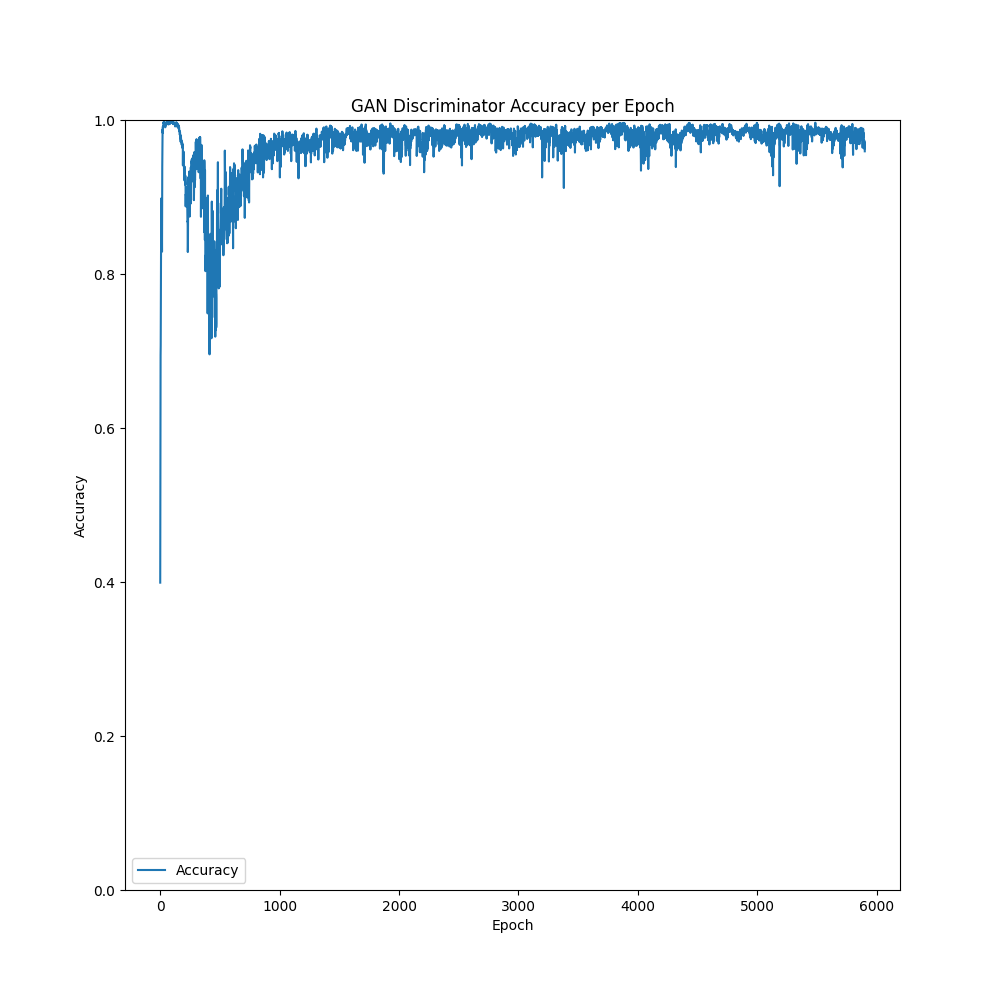
\includegraphics[width=0.49\textwidth]{img/2021_01_31_22_56_40_pianoroll-DC-GAN_GAN_Accuracy_per_Epoch_epoch_5900.png}
		\label{fig:pianoroll-acc}
	}
	\caption{Loss and accuracy during training of LSTM-based GAN}
\end{figure}

The results from this process were very satysfying. You can see and hear rythm in drums (red channel) and also repeating patterns and chords in instrumental channels (see figure \ref{fig:pianoroll-example})


\begin{figure}[h!]
	\centering
	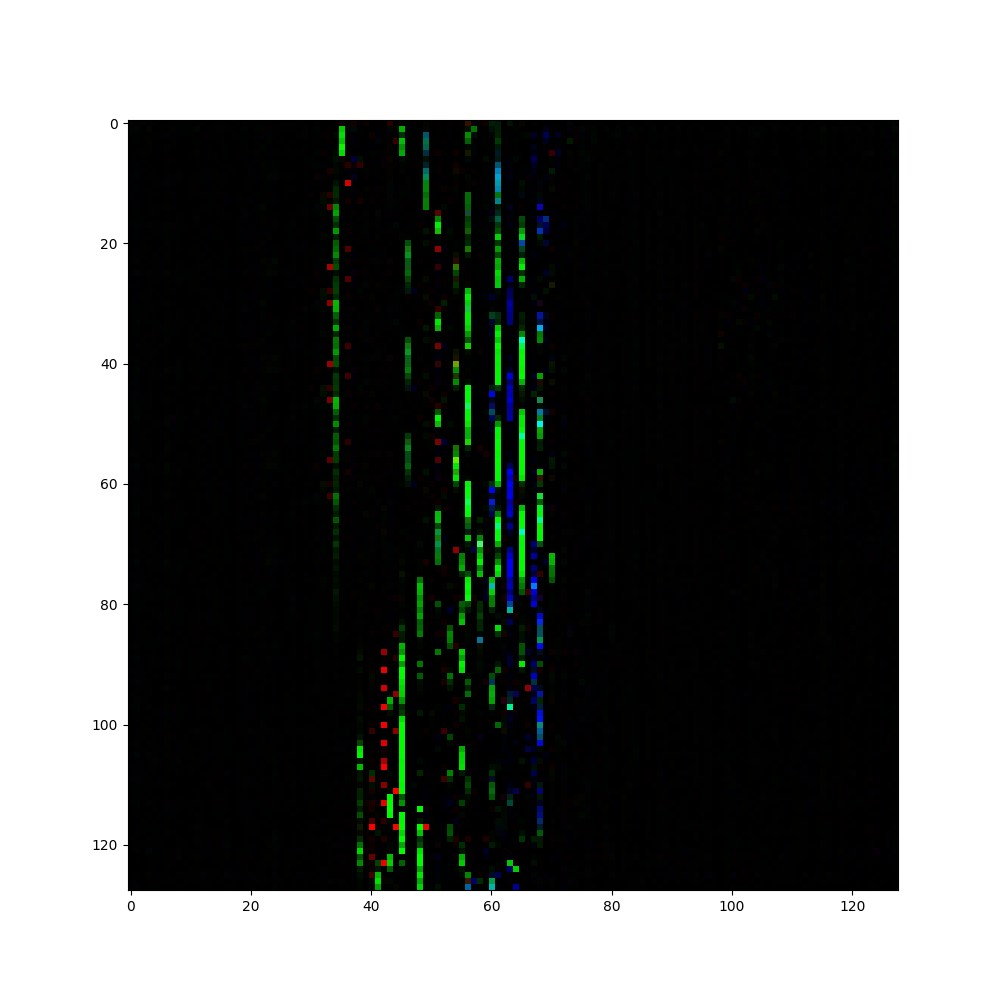
\includegraphics[width=0.69\textwidth]{img/2021_01_31_22_56_39_pianoroll-DC-GAN_epoch_5900.png}
	\caption{Loss and accuracy during training of LSTM-based GAN}
	\label{fig:pianoroll-example}
\end{figure}

\subsubsection{Others}

During my experiments I also tried to implement a system that would process sound in a form of spectrogram created from WAV file by short-time Fourier transform and converting it back to a WAV file, but the images to be processed were very large. The neural networks capable of processing such images could not be handled by my machine.

\clearpage

\section{Implemented software}

In order to prepare training and generation scripts I used the following tools:

\begin{itemize}
	\item Python 3.8
	\item Tensorflow and CUDA as training tool
	\item Keras as a library for building neural networks
	\item mido and pypianoroll libraries for processing MIDI files
	\item matplotlib library for visualization
	\item argparse library for handling command line interface.
\end{itemize}

Instructions for both training and generation scripts can be found in readme.md file in the repository.

\section{Summary}

As a result of the project I managed to deliver a intelligent information system that is capable of generating music. I did not expect spectacular results from a rather small system trained on my PC, since it requires a lot of computations, but what I managed to deliver is a satysfying result.

\bibliographystyle{plain}
\bibliography{bibliography.bib}

\end{document}
